% Chapter 1

% variables
\newcommand{\pdirone}{chapters/plots/chapter1}

% cross references

\chapter{Why Dark Matter?} % Main chapter title
%\chapter{Introduction} % Main chapter title

\label{chapter1}

Physics is a wonderful thing, I was always mesmerized by its ability to describe what surround us in a powerful and compact way, ultimately using this knowledge for the betterment of the mankind. When I was young, equations were like an ancient magic language to me. I was not able to understand it yet, but I was absolutely impressed by knowing that people that could, were able to control power that for a kid look like beyond any form of comprehension, from making incredibly heavy object flying faster than any bird, or destroying entire city by splitting something invisible for the naked eye. I always dreamed at some point to become part of this exclusive club of magician, and now that I am, I have to say: I got it all wrong! Physics requires a lot of thinking, a lot of reading, a lot of trial and error, in one word? A lot of work! What follows is my attempt to make a lasting contributes to this amazing field. It won't go to history, but I hope it will be important for some students that follow the scientist step, for sure it will be important to me.

So what is this thesis about? Dark Matter, if I had to use one word. One of the most prominent puzzle in all physics. With all our powerful and extremely precise models, we still have to explain more than 96\% of the matter in our universe. That is embarrassing! How could we miss all that? Turns out is not simple at all, when the matter that you are searching for stubbornly refuse to interact with your detectors, but I am sure that eventually physics will prove to be even more stubborn in their measurement, and eventually crack the code. This thesis was an attempt to this, an experiment to produce this elusive matter directly, in the attempt to measure its property. Since my group does not have a noble price in its hand, it must be no mistery that we did not yet succeeded, although this is not excluded for the future. I think the journey of me and the rest of my collegues is nevertheless very instructive, it is the typical story of how an experiment is born and conducted. An "happy ending" is not always expected, and should not be assumed by the scientist that is conducting the experiment, you are just there to observe, not decide. In my opinion, the experiment itself is the "happy ending" that a scientist is seeking, when it is well performed, and that is not depending on the final outcome of it. So with no further wait we can begin our journey, at the discovery of the NA64 experiment and its search of Dark Matter.

In this chapter our story begin, and as every story of science it begins with a mistery: Dark Matter. Why can't see it? Why can't we touch it? Those are not interesting questions, since many well understood phenomena can't be seen or touched. In the end it all boils down to one question: Why our models, that works so amazingly well in so many different situations, fail miserably in other situations apparently completely equivalent? This is what this chapter will be about, understand why we need the concept of dark matter, and justify what phenomena it could explain. Indeed one could think that is rather lazy to explain phenomena just by adding invisible matter in the system. "Just admit that you don't know what is going on!", is something that I heard myself when I try to explain my work to others. That is overall an honest question, an healthy scientific skepticism  about a theory that seems so arbitrary. In Sec.\ref{ch1:sec:dm-evidence} we will explore why we need this concept, and what are the alternatives to it. After that, we will come to realize that Dark Matter is a very simplistic term, that hides an extremely large number of possibilities that can be constructed using the framework of Quantum Field Theory (QFT). Dark Matter candidates are indeed very numerous, potentially even infinite, but we can focus on the most reasonable ones, that do not require extremely complicate model. In agreement with the scientific method, we try to extend our theory minimally, to see if it works, and only after we fail we add more complexity to our new model. In Sec.\ref{ch1:sec:dm-candidates} we will give a small review on these possibilities, trying to be succint but complete. After that, we will introduce the framework of thermal Dark Matter, one of the most successful in describing the observed relic density in our cosmos, that has the indisputable advantage of relating the mass of the Lightest Dark Matter (LDM) candidates with the cross section of annihilation. After these introductions we will finally concentrate ourself to a more specific model, which is one of the main focus of this thesis: the $U'(1)$ model. This model postulates the existence of an additional $U(1)$ symmetry that generates a "Dark Sector" of particles amounting to the invisible matter. The gauge boson of this symmetry, that we will label $\DM$ through this thesis, has been know with the catchy name of Dark Photon, due to playing the equivalent role of the standard model photon in this new symmetry. This model allows also a cross-term that couples the new Dark Photon with its standard counterpart, effectively building a portal between the two sectors. This is excellent news! It means we can produce this type of matter using modern accelerator if such model is true, which allow us to perform a particle physics experiments to probe this model. But why this model should be better than the others? There is not an easy answer to this. From scientific point of view, a model is better than another if it is more powerful in explaining the reality of things. In a framework as complicate as cosmology however, there are countless models that are equivalent in describing reality, which is why so many Dark Matter candidates exist. In a way, it is unavoidable that we share the work and probe all models one by one. However, sometimes a model can solve more than one problem at the same time, which would make them especially attractive for scientist. Originally, the Dark Photon was also an excellent explanation of the measured value of the anomalous muon magnetic moment, that to date deviates substantially (by 3.5 standard deviation) from the prediction of QED. We now know that such explanation is ruled out, since NA64 together with other experiments excluded it. Another interesting phenomena that could be explained is the so called $\DMX$-anomaly, originally known with the name of $^8$Be-anomaly. This name refers to an anomaly detected in the nuclear decay spectrum of Beryllium that would be justified by the existence of a particle not present in the standard model. This anomaly was later confirmed in the $^4$He atom as well, which makes it a very interesting phenomena to study. In Sec.\ref{ch1:sec:dm-u1model-motivations-x17} a review of this phenomena will be given. To avoid confusion, we point out here that the $\DMX$, which is the name given to the particle advocated to explain the observed anomaly, is not by definition a Dark Photon, since it posses some properties that are not present in a more vanilla model. However, its characteristic are similar enough to be probed by the NA64 experiment, as it will be clear from this thesis.

This chapter is meant to just answer the question: what are we searching for? This is the beginning of every scientific experiment, but arguably the easiest part! Building an experiment to produce the Dark Photon is the next step, which will be covered in chapter \ref{chapter2}. Turn a photon in a Dark Photon using this portal is however meaningless if we can't prove that we did it! A robust analysis method of the data collected need to be performed for this purpose, this is what we will explore in chapter \ref{chapter3} step by step, from the method to the selection criteria. In chapter $\ref{chapter4}$ we will than provide what most scientist are here for, the results! No Dark Matter has been found yet, but the data acquired allow us to exclude some specific models from being allowed credible explanation of reality. To reiterate an example already used: we now know thanks to this data, that the anomalous magnetic moment of the muon cannot be explained exclusively bu the $U'(1)$. The NA64 experiment is however far from over! The break given by the LHC long shutdown (and unfortunately by the recent rise of Covid-19 as well) allowed us to stop for a second a look for ways to improve our setup for the upcoming challenges of 2021! The knowledge we gained for the background and the experimental condition are used to design the new version of the setup to acquire a larger number of particles and thus probe a larger number of models. In chapter \ref{chapter5} we will review all these changes, in particular the new setup for the visible mode of 2021, that was the last project of my PhD, and that will use to hopefully find (or else exclude) the $\DMX$.

With no further wait, let's embark ourselves in this journey!

%----------------------------------------------------------------------------------------

\section{Evidence for Dark Matter}
\label{ch1:sec:dm-evidence}

The story of Dark Matter and the birth of this term is interesting on its own, and a good example of "unequivocal accumulated evidence" in science, but in a way is even more than that \cite{hooper, deSwart:2017heh}. The terms was first used in 1937 by astronomer Fritz Zwicky\footnote{Some weaker claim of a discrepancy were done even before by Knut Lundmark in 1930.} to justify the velocity dispersion in Coma cluster galaxies, which were deviated significantly from what predicted by simply asserting the mass from the visible matter. This hypothesis was discussed more seriously on in 1950, when astronomical surveys confirmed this results with high precision. This sparked an heated debate in the scientific community, and understandably many solutions to this problem did not include additional unknown matter, but rather modification of gravity or more sophisticated arguments based on dynamical equilibrium of such galaxies. In 1970 with the rising of radio astronomy the rotation curved of galaxies are studied in detail, and two studies performed by Kenneth Freeman and Vera Rubin separately confirm that the velocity or rotation of objects in a galaxy becomes flat at sufficient distance from its center. The idea becomes very influential to the cosmological community thanks to two very influential paper in 1974 by Einasto and Ostriker, that clearly states that the mass of galaxies has been underestimated by a factor 10 until then \cite{EINASTO1974,1974ApJ...193L...1O}. This was further strengthen by the end of the decade by very similar analysis, and well summarized in this review \cite{annurev.aa.17.090179.001031}. The existence of Dark Matter becomes more and more accepted in the years to come, both alternative theory also arise to explain observation without the need of additional matter. Pheraps the most famous today remains the MOND theory, theorized as a weak-field approximation of some more general theory of gravity yet to be discovered. Despite some early success, this theory has always proven to be challenging to merge in the general relativity framework, and is insufficient to justify some specific phenomena like the famous "bullet cluster", that is on the other hand very well explain by Dark Matter \cite{Clowe_2006}.

So what is the current situation of Dark Matter? Today the theory is well accepted in the scientific community, although some debate and alternative theory are still present, the existence of Dark Matter is the leading paradigm to explain all discrepancy observed \cite{hooper}. Outside from the compelling arguments listed above, advances in the field of cosmology and measurements technique have provided many other evidence that aid Dark Matter existence. For example gravitational lensing, in particular in the context of weak lensing, was used to characterize the mean distribution of Dark Matter and match it to the one predicted by large scale structure measurements \cite{weak-lensing}. The measurements of temperature anisotropies of the Cosmological Microwave Background (CMB) present structures compatible with Dark Matter, and well fitted in the $\Lambda$CDM model that we will introduce in Sec.\ref{ch1:sec:dm-thermal} \cite{Ade:2015xua}. On the top of this, many other arguments, including structure formation \cite{Navarro:1995iw}, baryon acoustic oscillation \cite{bao}, and Red-shift distortions \cite{Peacock2001} have proven consistently in agreement with Dark Matter existence and in particular with the $\Lambda$CDM model.

So let us assume like the majority of scientific community that Dark Matter indeed exist, what is it the exact nature? Can we point down some characteristic and a space of parameter that defines it exactly? Those are the questions that will be answered in the next section.

\section{Dark Matter candidates}
\label{ch1:sec:dm-candidates}

The first to ask ourselves is what kind of property Dark Matter should have to satisfy the experimental constraint given by cosmology. Following the excellent book of Stefano Profumo \cite{Profumo:2019ujg}, we can define the following properties:

\begin{itemize}
\item \textit{Dark}: Trivially enough, Dark Matter should not emit light, but a tiny charge is still compatible with data, which justifies models with "milli-charges" particles. What is effectively constraint is the ratio of charge to some power of the mass.
\item \textit{Collisionless}: Dark Matter self-interaction to mass ratio is constraint by observation of cluster mergers and the ellipticity of galactic halos. The cross-section itself is not however necessarly small, assuming a mass similar to the one of a proton, indeed the constraint amount to a cross section in the order of barn, very similar to the one observed for strong interaction.
\item \textit{Classical}: Dark Matter is observed to be confined on the galactic scales of a few kpc in dwarf galaxies. Hence, their de Broglie length must be smaller than that to have a coherent Dark Matter halo. This argument is typically used to put a lower limit on the DM mass. If the Dark Matter candidates is a fermion, constraints are stronger as Pauli blocking limits the density to at most the phase space density to $f=gh^{-3}$ where g are the number of internal degrees of freedom.
\item \textit{Fluid}: For macroscopic DM, with mass much larger than the solar mass $M_{\odot}$, tidal disruption is expected to break the stability  in global cluster. This limit is typically placed around $10^6 M_{\odot}$.
\end{itemize}

In summary, while the cosmological and Galactic Dark Matter density is known to a good degree, very weak constraint exist on the interaction strength and the exact mass of Dark Matter. The huge mass scale that spans over the possible region is excellently depicted in Fig.\ref{fig:dm-mass-range}, where we see several possible DM candidates in relation with their possible mass and search technique to probe them. A few experimental anomalies are labeled in red to see mismatch between theory and experiment that could potentially be explained by Dark Matter. We can see that most of them are in the \mev-\gev scale, which is the one covered by our experiment. Even problem of the cosmological scale, like small-scale structure, are potentially well explained by this class of models \cite{battaglieri2017cosmic}.

\begin{figure}[bht!]
  \centering
  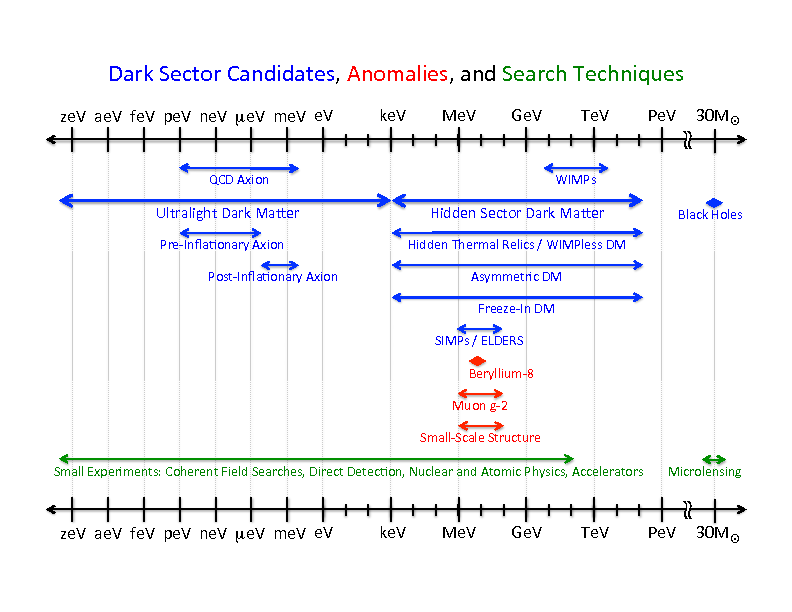
\includegraphics[scale=0.5]{\pdirone/DM_summary.png}
  \caption[Mass range for Dark Matter]{Mass range for Dark Matter and mediator particle candidates, experimental anomalies, and search techniques \cite{battaglieri2017cosmic}.}
  \label{fig:dm-mass-range}
\end{figure}

Because of the relatively loose constraint, it comes to no surprise that a vast amount of models have been theorized for the explanation of DM. The ones depicted in Fig.\ref{fig:dm-mass-range} are only a subset of what is possible, most of time by changing cleverly the model you can make it survive in scales were originally the model was not covered. It is the case for Axion Like Particles (ALPS), that are an extension of the QCD Axion model originally developed to solve strong CP problem \cite{PhysRevD.16.1791}. Contrary to Axions, their mass $m_a$ is taken as independent parameter from their main coupling $g_{a \gamma \gamma}$, and can be arbitrary large. Indeed this mass can also be in the \mev-\gev scale, in the range where the NA64 experiment is sensitive. As we will show in Sec.\ref{ch4:sec:exclusion limits}, we already used out data to constraint a portion of this parameter space \cite{Banerjee:2020fue}.

This thesis does not aim to cover in detail each model of Dark Matter, which is a subject worth a thesis of its own. The avid reader can take a look the following reviews for this purpose \cite{battaglieri2017cosmic,Profumo:2019ujg,HAMBYE2020135553,alex2016dark,review-particle-physics,Feng:2010gw}. Here, we provide a short description of the mainstream possibilities currently considered for Dark Matter:
\begin{itemize}
\item \textbf{\textit{WIMP}}: For a long period of time, Weakly Interacting Massive Particles (WIMP) were considered the most probable candidate by the scientific community. Their main characteristic is tree-level interaction with the W and Z boson, but not with gluons or photons. Historically, their mass is in the 10 \gev-\si{\tera\electronvolt}, although more recent models extended the mass range to lower masses as well. The so-called WIMP miracle \cite{Chang:2013oia}, provided a very effective and natural way to introduce Dark Matter in the thermal history of the early universe in a way that predicted to a very good degree the current relic density. However, after an extensive amount of research, accelerators and direct search have to this date failed to provide evidence to their existence \cite{Arcadi:2017kky}. These models have yet to be ruled out completely, and the remain to this date the most studied type of Dark Matter.
\item \textbf{\textit{Axions}}: Axion and Axion-like particles are obtained by introducing a new pseudoscalar field $a$ with coupling to photons \cite{Marsh:2015xka}. Originally Axions were motivated by the strong CP problem and they were predicted to be extremely light ($<$\si{electronvolt}). The model was later extended to offer a possible explanation for Dark Matter at higher masses. Several experiment based on the "light shining through a wall" concept or using a magnetic helioscope \cite{annurev.nucl.56.080805.140513} already put some stringent limits on Axions. Axion-like particles on the other hand can have a mass large enough to allow testing using accelerators.
\item \textbf{\textit{Sterile Neutrino}}: While Standard model neutrinos are not a good fit to explain Dark Matter as the are produced very hot in the early thermal bath, Sterile neutrinos are on the other hand a viable explanation. Models for this particle vary greatly, and some of the most attractive, like the ones that explain the light neutrinos masses as consequence of the \textit{see-saw} mechanism, are not a viable explanation for Dark Matter \cite{Feng:2010gw}. Nevertheless, models that explain observation do exist, and can be probed by direct detection experiments. To date, no credible signal has been observed.
\item \textbf{\textit{Dark Sector}}: By the name of Dark Sector, we describe a very large class of model characterize by particles not charged directly under strong, weak, or electromagnetic force \cite{alex2016dark}. Particles can still interact with the SM particle through additional interactions constraint by symmetry of the standard model. This are typically called "portals" interactions. This class of models, specifically the ones charged under a new U'(1) symmetry, are the focus of the NA64 experiment, and they will be described more in detail in Sec.\ref{ch1:sec:dm-sector}-\ref{ch1:sec:dm-u1model}
\end{itemize}

In this thesis, the class of models known as Dark Sector will be the focus. To build an experiment it is indeed instructive to focus on a particular signature predicted by a specific mode, in our case the U'(1) model. However, the opposite can still apply, i.e. a specific signature can turn out to be useful to constraint model not in the original scope of the experiment. It the case for the Axion-like particle, that are constraint by the NA64 experiment even though the original goal was to probe the Dark Photon. In summary, one should not think about the data produced by NA64 as exclusively powerful to constraint a single model, but should them freely in the broader framework of new physics.

\subsection{Thermal Dark Matter}
\label{ch1:sec:dm-thermal}

\subsection{The Dark Sector}
\label{ch1:sec:dm-sector}

Dark sectors , introduced in Sec.\ref{ch1:sec:dm-candidates}, are very interesting candidates to explain the origin of Dark Matter (see \cite{battaglieri2017cosmic,alex2016dark} for recent reviews). On the top of reproducing the observed DM abundance in freeze-out or freeze-in scenarios, many experimental anomalies currently observed can be explained inside this framework. The anomalous magnetic moment of the muon \cite{blum2013muon}, the proton charge radius \cite{Pohl2010} and more recently the $\DMX$-anomaly \cite{Krasznahorkay:2015iga,Krasznahorkay:2019lyl} have been suggested as possible hints of a dark sector \cite{alex2016dark}. The definition of this sector is extremely broad, and can accommodate many different models. Its physics however, can be explored effectively and in a systematic way by using specific portal interaction as classification scheme.  The existence of a mediator acting as a portal is not necessary in the Dark Sector, but it natural to select such models in the context of particle physics experiment, as they will be the one with some detectable signature\footnote{If we want to use these models to explain experimental anomalies on the other hand, the existence of a mediator becomes a necessity!} \cite{prw, pospelov}. The gauge and Lorentz symmetries restricts the ways in which the mediator can couple to SM particles. We can classify them using their spin and parity, and by excluding dimension operators larger than 5 we obtain four renormalizable possibilities \cite{alex2016dark}:

\begin{equation}
  \label{eq:dm-portals}
  \mathcal{L} \quad \supset \quad
\begin{aligned}
  &-\frac{\epsilon}{2 \cos{\theta_W}}B_{\mu \nu}F'^{\mu \nu}, &\textrm{vector portal}\\
  & (\mu \phi + \lambda \phi^2)H^{\dagger}H, &\textrm{Higgs portal}\\
  &y_n LHN, &\textrm{neutrino portal} \\
  &\frac{a}{f_a} F_{\mu \nu} F^{\mu \nu}, &\textrm{axion portal}
\end{aligned}
\end{equation}

In this work, we will limit the discussion on the vector portal, as it is the most viable for thermal models of LDM. If we assume the DM mediator to be a vector boson arising from an additional U'(1) gauge group under which the LDM is charged, we can derive a term $\epsilon / \cos{\theta_W} B^{\mu \nu} F'{\mu \nu}/2$ that is invariant both on this symmetry and the well known U(1) from QED. This model can be used to explain the phenomenology of a large class of models, such as scenarios where the Dark Photon couples preferentially to Baryonic, leptonic, or (B - L) currents. One such case, where the coupling to Baryon is disfavored, is the protophobic $\DMX$ gauge boson \cite{PhysRevD.95.035017}. Additionally, the DM could also have a Majorana couplings to the mediator \cite{PhysRevD.93.063523}, or it could live in a rich sector \cite{Morrissey_2014}.

From here on we will shift the discussion on more practical terms, which means describing a minimal model of dark gauge vector boson and calculate its yield in a particle physics experiment. This model can be easily extended to more complex scenario by adding constraint and terms on the Lagrangian. We remind here, that today the progress on experimental results started to put heavy constraint on this parameter space, thanks as well to the NA64 efforts, excluding even important models like the one capable of justifying the anomalous magnetic moment of the muon. This constraint have been placed by beam dump \cite{jdb, charm, rio, e137, konaka, bross, dav,  ath, nomad, e787, essig1, blum,sg1, blum1, sarah1}, fixed target \cite{apex,merkel,merkel1}, collider \cite{babar, curt, babar1}, rare particle decay searches \cite{sindrum, kloe, sg2, kloe2, wasa, hades, phenix, e949, na48, pol, kloe3} and the new determination of the fine structure constant $\alpha$ combined with the measurement of $(g-2)_e$ \cite{Parker191,PhysRevLett.100.120801}.

\section{The U'(1) model}
\label{ch1:sec:dm-u1model}

To build a minimal model of the Dark Sector, we choose the vector portal described above, which add an additional vector gauge boson called Dark Photon, that in this work we will label as $\DM$\footnote{The field will be labeled in the same way for for commodity.}. The new U'(1) symmetry adds terms to the standard model Lagrangian in the same fashion of the U(1) symmetry of QED. We obtain:

\begin{equation}
  \label{eq:dm-lagrangian}
  \mathcal{L}_{DS} = \mathcal{L}_{SM} \underbrace{- \frac{1}{4}F'_{\mu \nu}F'^{\mu \nu} + \frac{m_{\DM}}{2}A'_{\mu}A'^{\mu}} + i \bar{\chi} \partial_{\mu} \chi - m_{\chi}\bar{\chi}\chi - e_D \bar{\chi}\gamma^{\mu}A'_{\mu}\chi
\end{equation}

Here we also added a Dirac spinor field $\chi$ that is coupled to $\DM$ by a coupling constant $g_D$. This is for the completeness of the model, which is also supposed to contain a LDM that justify the relic density. There are however other possibilities to a simple Dirac fermion, as will be seen in Sec.\ref{ch4:sec:exclusion limits}. The part of the lagrangian over parenthesis is the one generated by the new U'(1) symmetry and is the one of main relevance to compute the physic of the portal. In particular the terms multiplied by $\epsilon$ represent the kinetic mixing between $\gamma$ and $\DM$, as it multiplies the two field tensor generated by the two U(1) groups. Here $\epsilon$ is taken as an a priori parameter that controls the strength of the kinetic mixing. it can in principle have any value, but since it is naturally generated inside the loop of heavy fields charged under both symmetries, it is expected to be small, in the range $\epsilon \sim 10^{-8} - 10^{-2}$ \cite{jdb}. In terms of production rate in particle physics experiment, the model is completely characterized by only the mass of the mediator $m_{\DM}$ and the strength of the coupling $\epsilon$, and hence the parameter space of these hypothesis  is characterized by the plane $\dmplane$. The mixing terms generated the interaction:

\begin{equation}
  \label{eq:dm-interaction}
  \mathcal{L}_{int} = \epsilon e A'_{\mu}J'_{em}
\end{equation}

between the Dark photon and the ordinary matter. In NA64, the Dark Photon is produced as "Dark Bremsstrahlung" in the process $e^- Z \to e^- Z \DM(\DM \to \textrm{decay})$. Calculate this cross-section is challenging due to complicate integral involving nuclear effects. We instead assume that the mass of $\DM$ is large enough to treat the $\gamma$ exchanged in the reaction as physical, which allows us to reduce the problem to the scattering of the electron with a physical photon emitted by nucleus. This is called the Weizsacker Williams (WW) approximation \cite{Kim:1973he}, and yields to the result:

\begin{equation}
  \label{eq:dm-diff-cross}
  \frac{d\sigma}{dxd\cos{\theta_{\DM}}} = \frac{8 Z^2 \alpha^3 \epsilon^2 E^2_0}{\textrm{U}^2} \mathcal{L}og \times \left[ (1 - x + x^2/2) - \frac{x(1-x)m^2_{\DM}E^2_0 x \theta^2_{\DM}}{\textrm{U}^2} \right]
\end{equation}

Here, $E_0$ is the energy of the incoming electron, $E_{\DM}$ is the energy of the emitted $\DM$, $\theta_{\DM}$ is the angle of emission in the lab frame, and Z is the atomic number of the nucleus. $x=E_{\DM}/E_0$ is the fraction of original energy transfered to the Dark Photon, the $\mathcal{L}og$ is a factor accounting for atomic screenings and nuclear size effects, numerically $\mathcal{L}og \sim 5 - 10$. The function U defines the virtuality of the incoming electron in the intermediate state of the Bremsstrahlung, defined as:

\begin{equation}
  \label{eq:u-func}
  \textrm{U} = E^2_0 x \theta^2_{\DM} + m^2_{\DM} \frac{1 - x}{x} + m^2_e x
\end{equation}

We perform the angular integral on Eq.\ref{eq:dm-diff-cross}:

\begin{equation}
  \label{eq:dm-diff-cross-int}
  \frac{d\sigma}{dx} \approx \frac{8 Z^2 \alpha^3 \epsilon^2 x}{m^2_{\DM}} \left( 1 + \frac{x^2}{3(1-x)} \right) \mathcal{L}og 
\end{equation}

Now we can finally apply this formula do compute the yield inside a target. If we assume an electron with energy $E_0$ impacts a thick target with radiation length $T$, we derive:

\begin{equation}
  \label{eq:dm-general-yield}
  \frac{dN}{dx} = N_e \frac{N_0 X_0}{A} \int_{E_{\DM}}^{E_0} \frac{dE_1}{E_1} \int_0^T dt I(E_1;E_0;t) \times E_0 \frac{d\sigma}{dx'}\Big|_{x' = E_{\DM}/E_1}
\end{equation}

Here, $N_0$ is the Avogadro's number, $X_0$ is the radiation length of the target, A is the target atomic mass, and I is the energy distribution of electrons after passing through t radiation length. The above integral is still fairly complicate, mainly an accurate description of the electron energy distribution after t radiation length is not an easy task\footnote{In practice, this is solved by MC-simulation as we will see in chapter \ref{chapter3}}. A common approach is the thin target approximation, where $I \approx \delta (E_1 - E_0)$ since the target is assumed to be thin enough that no em-shower is triggered. However, we will see that is very desirable to block the incoming $e^-$ completely in a realistic experiment, which means a thick target should instead be used. This requires some additional care in parametrizing I, which is illustrated in Appendix.\ref{appA:sec:cross-section}. Here we simply jump to the final results, the rate at which the $\DM$ is produced is approximated by:

\begin{equation}
  \label{eq:dm-rate}
  N_{\DM} \sim N_{EOT} \times C' \epsilon^2 \frac{m_e^2}{m^2_{\DM}}
\end{equation}

Which gives us an excellent formula to calculate the number of Dark Photon produced as function of the EOT\footnote{Electron On Target} accumulated. Here $C'$ accounts for all factors outside the one relevant for the specific model, and it numerically $C' \approx 10$. One has to be careful with this formula, since many approximation were used to derive it and is expected to be accurate only within an order of magnitude \cite{jdb}. However, it provides us with some vary useful scaling with the parameters of the model, and allow us some simple reasoning on how to the sensitivity of the experiment plotted in the $\dmplane$ space will look like. To compute the exact sensitivity with high precision, a detailed MC-simulation is typically used instead, which will be detailed in Sec.\ref{ch3:sec:geant4}.

\subsection{Decay modes}
\label{ch1:sec:dm-decay}

Producing $\DM$ is not sufficient if we have no way to understand if the interaction happened. The next step would be to devise a mechanism to detect the emission. To answer this question, it is important to understand what happens to $\DM$ after is emitted inside the target. We remember that in our model a Dirac field is also present, so the Dark Photon can in principle decay in a pair of particles generated by this field, which are stable Dark Matter particles that account for the relic density. However a decay in leptons from the Standard Model is also possible, since the kinetic mixing mechanism can act in both directions. This provide two different channel for decay, that we will see are of extreme importance to decide for a precise detection strategy. Inside the QFT framework, is easy to compute both branching ratio, as detailed in Appendix.\ref{AppendixA}. Here we provide the final answer:

\begin{equation}
  \label{eq:dm-bratio}
  \begin{aligned}
    &\Gamma(\DM \to \bar{\chi} \chi) = \frac{\alpha_D}{3} m_{\DM} \left( 1 + \frac{2m^2_{\chi}}{m_{\DM}^2}\right) \sqrt{1 - \frac{4m_{\chi}^2}{m^2_{\DM}}}\\
    &\Gamma(\DM \to l^+l^-) = \frac{\alpha \epsilon^2}{3} m_{\DM} \left( 1 + \frac{2m^2_{l}}{m_{\DM}^2}\right) \sqrt{1 - \frac{4m_{l}^2}{m^2_{\DM}}}
  \end{aligned}
\end{equation}

For completeness, the visible mode decay is written in a general way that accounts for a general lepton. By looking at the lepton of the standard model, it is clear that only the decay $\aee$ will be relevant, since for muons it is suppressed by a factor $(m_e/m_{\mu})^2 \approx 10^4$ and no Dark Photon in the range of collider experiment has enough mass to decay into a tau.

Here again we can investigate two different regimes:
\begin{itemize}
\item \textbf{\textit{Invisible decay regime}}: If $\alpha_D \gg \alpha \epsilon^2$, the branching ratio of the invisible decay is dominant, hence the Dark photon will always decay $\DM \to \bar{\chi} \chi$. This decay is characterized by missing momentum inside the target, as the $\dmchi$ cross-section of interaction is extremely low. One could put a detector to measure such interaction, but this would happen with a chance of $\sim \alpha_D \epsilon^2$ for a total rate of $N_{\DM} \sim \epsilon^4 \alpha_D$, much lower than what presented in Eq.\ref{eq:dm-rate}. In NA64, missing energy is used to characterize this decay channel. 
\item \textbf{\textit{Visible decay regime}}: If $\alpha_D \ll \alpha \epsilon^2$, the branching ratio of the visible decay is dominant, specifically the decay $\aee$. The Dark Photon will travel for a short time without interaction, and then decay into a $\ee$ pair. No missing momentum in this case is observed, but if the target is taken enough thick to block completely the incoming electron, the $\DM$ will provide a channel to penetrate the target and decay immediately after, generating an event not predicted in the SM. This concept is similar to a "Light shining through a wall" experiment popular for Axion searches, with the differences that is not a $\gamma$ but a $\ee$ that appears after the wall.
\end{itemize}

The two channels justify different phenomenology and are interesting in their own sake. The NA64 experiment aims to cover both of them, with slightly different setups to accommodate their different phenomenology. Before going into the detail, one can ask if the two decay channel above contributes some way in the total rate computed in Eq.\ref{eq:dm-rate}. The answer to this question is yes! Here we will give a quick reasoning on why that is the case, and correct the formula accordingly.

In the case of the invisible decay, the signature is missing momentum in our setup. Producing the $\DM$ seems to be enough to detect it, as there will always be missing momentum as long as a Dark Photon is emitted. While this is true, one could ask what amount of missing momentum is needed to be noticeable in the apparatus. The actual fraction of energy missing requires for a signal event in NA64 is $E_0/2$, i.e. half of the original beam energy. The answer to why this value is chosen is not trivial, and requires proper accounting of the background, which will be given in Sec.\ref{ch3:sec:bkg}.  For now we just realize that our rate need to be corrected by integrating the cross section only to a specific energy value in Eq.\ref{eq:dm-general-yield}. It is clear from Eq.\ref{eq:dm-diff-cross} that the cross-section is peaked for $x \sim 1$ for any values of $\dmplane$, hence this factor will be model independent. Some less trivial effects visible in MC-simulation might introduce some weak dependence on the exact model, but they can be in first approximation excluded. Hence, this additional steps just modifies slightly the numerical value of $C'$ in Eq.\ref{eq:dm-general-yield}, but does not introduce any additional scaling. In the case of invisible mode, this formula can still be used in good approximation to compute the final signal yield.

What about the visible mode? Like for the previous case, we can argue that a minimal energy should be required to punch-through the wall to be visible, and that will account as before to some additional factor to the rate. In this case however, the $\DM$ needs to travel outside the target to be visible, otherwise the $\ee$ will just be absorbed inside the material. To compute this effect, we first of all need to calculate the decay length of this particle in the laboratory frame.


\begin{eqnarray}
  L_{\DM} = \gamma c \tau \simeq \frac{3E_1}{m^2_{\DM}\alpha \epsilon^2} \simeq 28.3 ~{\rm mm}  \Bigl[\frac{E_{\DM}}{100~ {\rm GeV}}\Bigr] 
  \Bigl[\frac{17~ {\rm MeV}}{m_{\DM}}\Bigr]^2 \Bigl[\frac{10^{-3}}{\epsilon}\Bigr]^2
  \label{eq:dm-decay-length}
\end{eqnarray}

Where we negated the (small) phase space corrections and assumed only the $\aee$ is kinematically allowed. For the sake of argument, we assume that $\DM$ is emitted always at the beginning of shower with maximal energy $E_{\DM} = E_0$. The amount of $\DM$ that penetrate the wall can be computed by integrating the decay spectrum inside the fiducial-volume of the experiment, which starts from the end of the target and ends some place downstream. We can multiply this fraction to Eq.\ref{eq:dm-rate}, and obtain the signal yield expected for the visible mode:

\begin{equation}
  \label{eq:dm-rate-vis}
    N_{\DM} \sim \underbrace{N_{EOT}}_{\textrm{beam-intensity}} \times \underbrace{C' \epsilon^2 \frac{m_e^2}{m^2_{\DM}}}_{\textrm{cross-section}} \times \underbrace{\left(e^{- L_{dump}/L_{\DM}} - e^{-L_{fiducial}/L_{\DM}}\right)}_{\textrm{decay length}}
  \end{equation}

  Were we labeled each term by its source. Here again we can recognize two important limit in this equation, i.e. a decay length much shorter than the length of the fiducial volume $L_{\DM} \gg L_{Fiducial}$ or the other way around. Most of the parameter space interesting for NA64 is characterized by a length much smaller than the total decay volume. We can then exclude the second term of the decay length, we finally obtain:

  \begin{equation}
    \label{eq:dm-rate-vis-limit}
    N_{\DM}^{(\aee)} \sim N_{EOT} \times C' \epsilon^2 \frac{m_e^2}{m^2_{\DM}} \times e^{-k\frac{L_{dump} m^2_{\DM}\epsilon^2}{E_0}}
  \end{equation}

  This means that the signal yield is exponentially suppressed for large masses and couplings! Models with these properties will be exponentially more difficult to cover, and increasing the beam-intensity will only improve the sensitivity logarithmically. It so happens that a region of parameter space with these properties is also very interesting from the phenomenological point of view! An anomaly in the nuclear spectrum of a Beryllium isotope suggest that a particle with such properties might exist. As we will see in the next section, NA64 is sensitive to this hypothetical particle\footnote{A portion of this parameter space was already excluded by recent NA64 analysis \cite{Banerjee:2019hmi,Banerjee:2018vgk}.}, but the high coupling $\epsilon$ makes it hard to completely probe this model. The next section will give an overview of this particle, which remains to date one of the main goal of NA64 experiment.

\subsection{The X17 anomaly}
\label{ch1:sec:dm-u1model-motivations-x17}

A great boost to search for the new light boson weakly coupled to Standard Model particles was triggered by the recent observation of a $\sim$7$\sigma$ excess of events in the angular distribution of $\pair$ pairs produced in the nuclear transitions of the excited $^8$Be$^*$ nuclei to its ground state via internal $\ee$ pair creation \cite{Krasznahorkay:2015iga}. The latest results of the ATOMKI group report a similar excess at approximately the same invariant mass in the nuclear transitions of another nucleus, $^4$He \cite{Krasznahorkay:2019lyl}.

It was put forward  \cite{Feng:2016jff,PhysRevD.95.035017}, that this anomaly can be interpreted as the emission of a protophobic gauge boson $\DM$ decaying into $\pair$ pairs. To be consistent with the existing constraints, the $\DM$ boson should have a non-universal coupling to quarks and a coupling strength with electrons in the range of $2\times 10^{-4} \lesssim \epsilon_e \lesssim 1.4\times 10^{-3}$ which translates to a lifetime of the order of $10^{-14}\lesssim \tau_X \lesssim 10^{-12}$~s. Remarkably, this model also explains within experimental uncertainty the new result obtained with the $^4$He nucleus, providing both kinematical and dynamical evidence to support this interpretation \cite{Feng:2020mbt}. This model will be used as benchmark for the NA64 current results and to cast the sensitivity of the new setup described in this article. However, other solutions of the $\DM$ anomaly were proposed, see for example \cite{Nam:2019osu, Seto:2016pks}.

Interestingly, such a new boson with a relatively large coupling to charged leptons could also resolve the tension between measured and predicted values of the $(g - 2)_{\mu}$. In addition to vector and axial-vector explanation of the $\DM$ anomaly, one can consider scenarios involving hidden pseudo-scalar boson \cite{Ellwanger:2016wfe}. Corresponding pseudo-scalar couplings to electrons satisfy existing experimental constraints \cite{Andreas:2010ms,Adler:2004hp}. An analysis to probe such pseudo-scalar states at NA64 \cite{Kirpichnikov:2020tcf} would require a proper Monte-Carlo simulation of the spectra and flux of light pseudo-scalar boson produced in the target by electrons.
Another interesting result comes from the new measurement of $\alpha$ performed by Parker et al. \cite{Parker191} which combined with the $(g-2)_e$ measurements result in a 2.4$\sigma$ deviation from the QED predictions \cite{PhysRevLett.100.120801}. Should this tension be confirmed, the two constraints coming from the NA64 results and $(g - 2)_e$ would exclude the vector and axial vector couplings explanation of $\DM$. On the other hand, models with nonzero V$\pm$A coupling constant with the electron would explain both electron and muon $(g - 2)$ anomalies \cite{Krasnikov:2019dgh}. In these models, the $\DM$ could have a coupling of $6.8\cdot 10^{-4} \lesssim \epsilon \lesssim 9.6 \cdot 10^{-4}$ which leaves an interesting region of the parameter space to be explored.
These models motivated the study of the phenomenological aspects of such a light vector boson weakly coupled to quarks and leptons (see, e.g., Refs.~\cite{fayet1, fayet2, fayet3, fayet4,jk, cheng, Zhang:2017zap, ia, liang, bart}) 
and new experimental searches (see e.g., Refs.~\cite{battaglieri2017cosmic, nardi}).

Recently, the NA64 collaboration has reported new results that excluded the $\DM$ boson  with the coupling strength  to electrons in the range $1.2 \times 10^{-4} < \epsilon_e < 6.8 \times 10^{-4}$ \cite{Banerjee:2018vgk,Banerjee:2019hmi}, by using the calorimeter technique proposed in \cite{Gninenko:2013rka,Andreas:2013lya}. The remaining region of parameter space $6.8 \times 10^{-4} < \epsilon < 1.4 \times 10^{-3}$ is extremely challenging to probe in the current setup. The reason for this is the high coupling of this region that suppress exponentially the signal yield due to the low decay length. We can observe this by inverting Eq.\ref{eq:dm-rate-vis} and transform it into an expression to probe different value of $\epsilon$. If we define $\epsilon_{\textrm{up}}$ as the maximum $\epsilon$ that can be probed with a given set of data and we absorb all the constant in $C'$ we find:

\begin{equation}
  \label{eq:x17-coverage}
  \epsilon_{\textrm{up}} \sim C' \times \frac{E_0}{L_{\textrm{dump}}m^2_{\DMX}} \times \log{\left(N_{EOT} \epsilon^2 \frac{m_e^2}{m_{\DMX}^2}\right)}
\end{equation}

Increasing the number of EOT only improve our limit logarithmically, and a quick computation shows that an unfeasible number $>10^{14}$ of event are needed to explore this region. On the other hand, changing the impact energy of the length of the dump improve our limit linearly. A new setup was proposed to increase the signal yield while keeping the background under control (and in principle even reduce it) by decreasing the length of the target. The new setup is described in Sec.\ref{ch5:sec:new-vismode-setup}, and was shown to be able to cover fully the remaining region.


%%% Local Variables:
%%% mode: latex
%%% TeX-master: "../PhDthesis"
%%% End:
